\section{Durchführung}
Für den Versuch wird ein RC-Kreis mit integriertem Generator sowie ein Oszilloskop verwendet. Am Oszilloskop kann dabei der
Spannungsverlauf am Kondensator $U_C(t)$ abgelesen werden, während am Generator die Frequenz der anregenden Spannung reguliert wird.
Für die erste Messreihe wurde der RC-Kreis mit einer Rechteckspannung gespeist, sodass auf dem Oszilloskop jeweils Auszüge von Auf- und Entladevorgang 
zu beobachten sind. Aus diesen wird eine Aufladekurve gewählt und diese mit ca. $15$ Messwerten für Spannung und zugehörige Zeit ausgehend von einem 
selbstgewählten Ursprung abgetastet. \\
Anschließend wird am Generator eine Sinusspannung gewählt. Unter Variirung der Frequenz der anregenden Spannung wird am Oszilloskop
die Spitze-zu-Spitze-Spannung gemessen, um die Frequenzabhängigkeit der Amplitude zu untersuchen. \\
Zuletzt wird am Oszilloskop die Kondensatorspannung gemeinsam mit der anregenden Spannung angezeigt. Aus diesem Bild lässt sich, wiederum
unter Veränderung der Generatorfrequenz, die Phasenverschiebung beider Spannungen ablesen und so deren Frequenzabhängigkeit bestimmen.
Dies erfolgt wie in Abbildung \ref{fig:Phasenverschiebung} 
\begin{figure}
\centering
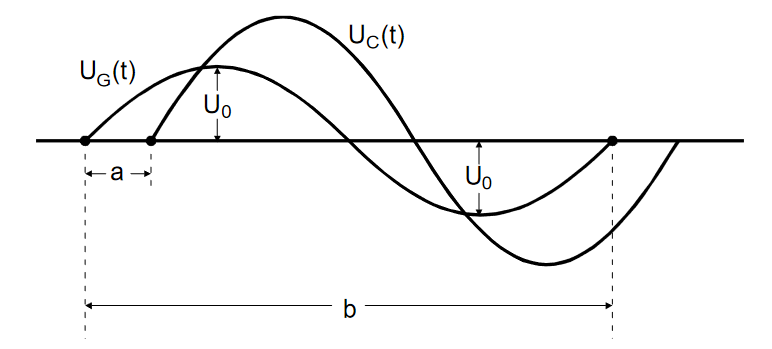
\includegraphics[width=8cm, keepaspectratio]{Phasenverschiebung}
\caption{Bestimmung der Phasenverschiebung}
\label{fig:Phasenverschiebung}
\end{figure}
woraus sich durch
\begin{equation}
\phi=\frac{a}{b}2\pi
\end{equation}
die Phasenverschiebung bestimmen lässt.
